\chapter{MOSFET and Amplifying Circuit}

\section{Classification of MOSFET}

\begin{figure}[H]
  \centering
  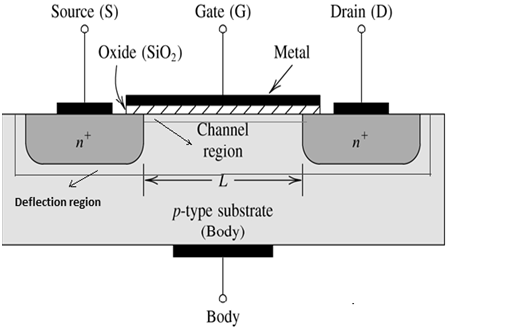
\includegraphics[width=0.5\linewidth]{figures/MOSFET-BLOCK-DIAGRAM.png}
  \caption{MOSFET Block diagram}
  \label{fig:}
\end{figure}

\subsection{N-type Enhancement-mode MOSFET}

\begin{figure}[H]
  \centering
  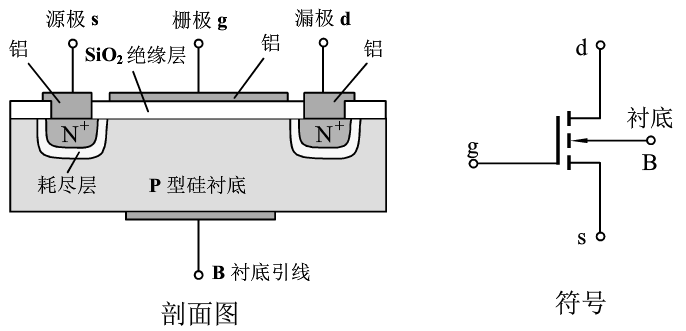
\includegraphics[width=0.7\linewidth]{figures/ENMOS}
  \label{fig:}
\end{figure}

Only when $V_{GS} > V_{TN} > 0$, N-Channel will be formed, MOSFET is conductive. $V_{TN}$ is called the Threshold Voltage.

\begin{figure}[H]
  \centering
  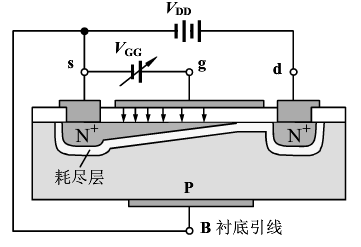
\includegraphics[width=0.5\linewidth]{figures/ENMOS2}
  \label{fig:}
\end{figure}

\begin{figure}[H]
  \centering
  \begin{subfigure}{.5\textwidth}
    \centering
    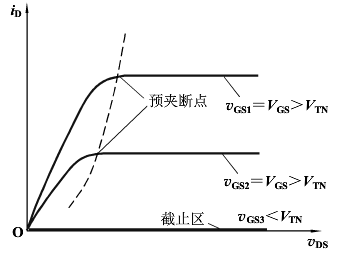
\includegraphics[width=\linewidth]{figures/ENMOSIV1}
    \label{fig:}
  \end{subfigure}%
  \begin{subfigure}{.5\textwidth}
    \centering
    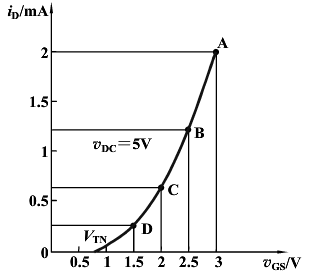
\includegraphics[width=\linewidth]{figures/ENMOSIV2}
    \label{fig:}
  \end{subfigure}
  \caption{The I-V Characteristic of N-type Enhancement-mode MOSFET}
  \label{fig:}
\end{figure}

\subsection{N-type Depletion-mode MOSFET}

The only difference between Enhancement-mode and Depletion-mode is the charges in oxide, which made $V_{TN} < 0$

\begin{figure}[H]
  \centering
  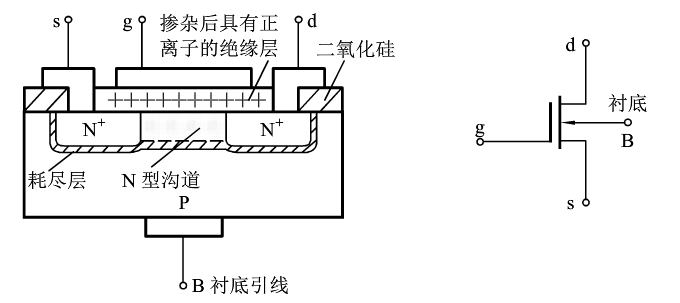
\includegraphics[width=0.7\linewidth]{figures/DNMOS}
  \label{fig:}
\end{figure}

\begin{figure}[H]
  \centering
  \begin{subfigure}{.5\textwidth}
    \centering
    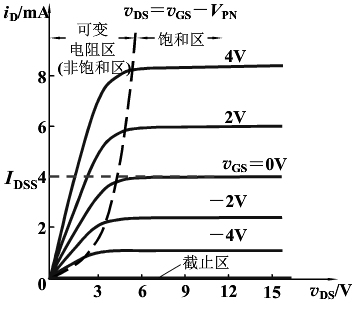
\includegraphics[width=\linewidth]{figures/DNMOSIV1}
    \label{fig:}
  \end{subfigure}%
  \begin{subfigure}{.5\textwidth}
    \centering
    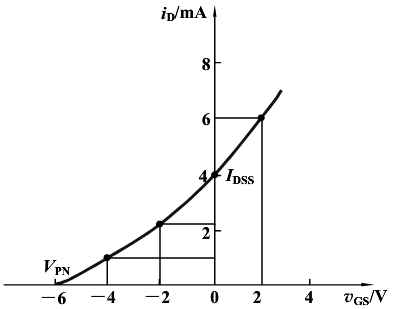
\includegraphics[width=\linewidth]{figures/DNMOSIV2}
    \label{fig:}
  \end{subfigure}
  \caption{The I-V Characteristic of N-type Depletion-mode MOSFET}
  \label{fig:}
\end{figure}

\subsection{P-type MOSFET}

\begin{figure}[H]
  \centering
  \begin{subfigure}{.3\textwidth}
    \centering
    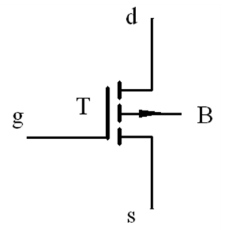
\includegraphics[width=\linewidth]{figures/EPMOS}
    \caption{Enhancement-mode}
    \label{fig:}
  \end{subfigure}%
  \begin{subfigure}{.3\textwidth}
    \centering
    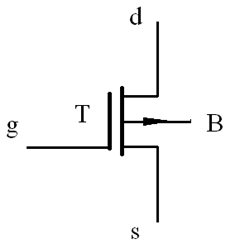
\includegraphics[width=\linewidth]{figures/DPMOS}
    \caption{Depletion-mode}
    \label{fig:}
  \end{subfigure}
  \caption{The Electronic Symbol of P-type MOSFET}
  \label{fig:}
\end{figure}

\begin{figure}[H]
  \centering
  \begin{subfigure}{.3\textwidth}
    \centering
    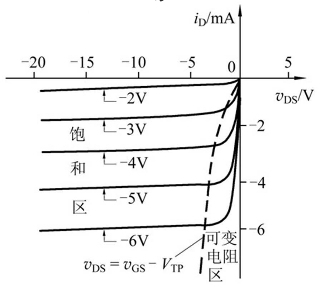
\includegraphics[width=\linewidth]{figures/PMOSIV1}
    \label{fig:}
  \end{subfigure}%
  \begin{subfigure}{.3\textwidth}
    \centering
    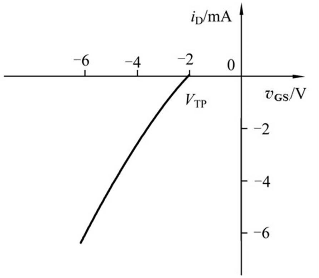
\includegraphics[width=\linewidth]{figures/PMOSIV2}
    \label{fig:}
  \end{subfigure}
  \caption{The I-V Characteristic of N-type Depletion-mode MOSFET}
  \label{fig:}
\end{figure}

\section{Static Working Point}

\begin{figure}[H]
  \centering
  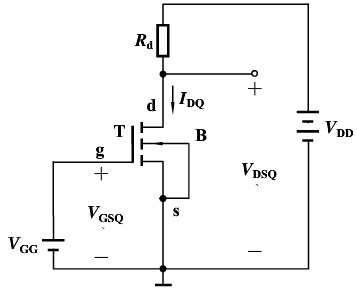
\includegraphics[width=0.5\linewidth]{figures/MOSFET-Static}
  \label{fig:}
\end{figure}

To calculate the static working point of a MOSFET

\begin{equation*}
  \left\{
  \begin{aligned}
    V_{GSQ} &= V_{GG} \\
    I_{DQ} &= K_n \left( V_{GSQ} - V_{TN} \right)^2 \\
    V_{DSQ} &= V_{DD} - I_{DQ} R_d
  \end{aligned}
  \right.
\end{equation*}

Note that $V_{DSQ} > V_{GSQ} - V_{TN}$ must be verified to ensure that MOSFET is working in active mode. Then for small AC signal, the current at drain is

\begin{equation*}
  \begin{aligned}
    i_D = 2 K_n \left( v_{GS} - V_{TN} \right) v_{GS} = g_m v_{GS}
  \end{aligned}
\end{equation*}

\section{Early Effect}

\begin{figure}[H]
  \centering
  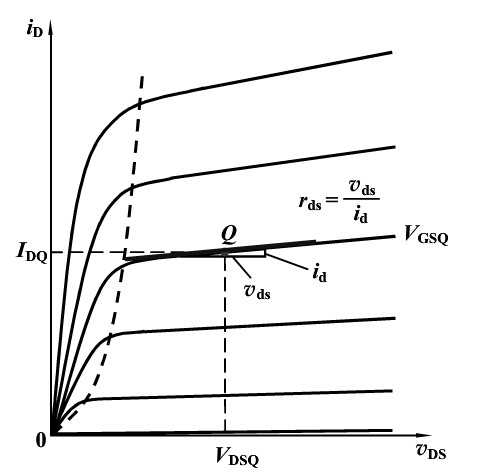
\includegraphics[width=0.3\linewidth]{figures/MOSFET-Early-Effect}
  \caption{MOSFET-Early-Effect}
  \label{fig:}
\end{figure}

\begin{equation*}
  \begin{aligned}
    i_D = K_n \left( v_{GS} - V_{TN} \right)^2 \left( 1 + \lambda v_{DS} \right)
  \end{aligned}
\end{equation*}

\begin{equation*}
  \begin{aligned}
    r_{ds} = \left. \dfrac{\partial v_{DS}}{\partial i_D} \right|_{V_{GSQ}} = \dfrac{1}{\lambda K_n \left( V_{GSQ} - V_{TN} \right)^2} \approx \dfrac{1}{\lambda I_{DQ}} = \dfrac{V_A}{I_{DQ}}   
  \end{aligned}
\end{equation*}

Where $V_A$ is called the Early Voltage

\begin{equation*}
  \begin{aligned}
    V_A = \dfrac{1}{\lambda} 
  \end{aligned}
\end{equation*}

\section{Three types of Amplifier Circuit}

\subsection{Common Source Amplifier Circuit}

\begin{figure}[H]
  \centering
  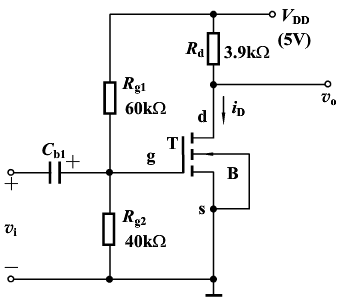
\includegraphics[width=0.5\linewidth]{figures/MOSFET-Common-S}
  \label{fig:}
\end{figure}

\begin{equation*}
  \left\{
  \begin{aligned}
    V_{GSQ} &= \left( \dfrac{R_{g2}}{R_{g1} + R_{g2}}  \right) V_{DD} \\
    I_{DQ} &= K_n \left( V_{GSQ} - V_{TN} \right)^2 \\
    V_{DSQ} &= V_{DD} - I_{DQ} R_tI_d
  \end{aligned}
  \right.
\end{equation*}

\begin{equation*}
  \begin{aligned}
    g_m = 2 K_n \left( V_{GSQ} - V_{TN} \right)
  \end{aligned}
\end{equation*}

\begin{figure}[H]
  \centering
  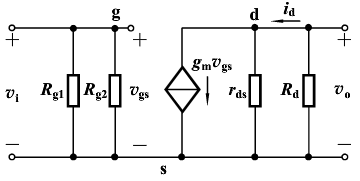
\includegraphics[width=0.5\linewidth]{figures/MOSFET-Common-Ss}
  \label{fig:}
\end{figure}

\begin{equation*}
  \begin{aligned}
    A_v = - g_m \left( r_{ds} \parallel R_d \right)
  \end{aligned}
\end{equation*}
\begin{equation*}
  \begin{aligned}
    R_i &= R_{gs1} \parallel R_{gs2} \\
    R_o &= R_d \parallel R_d \approx R_d
  \end{aligned}
\end{equation*}

\subsection{Common Drain Amplifier Circuit}

\begin{figure}[H]
  \centering
  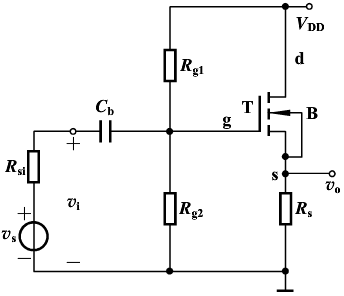
\includegraphics[width=0.5\linewidth]{figures/MOSFET-Common-D}
  \label{fig:}
\end{figure}

\begin{equation*}
  \left\{
  \begin{aligned}
    V_{GSQ} &= \dfrac{R_{g2}}{R_{g1} + R_{g2}} \cdot V_{DD} - I_{DQ} R_s  \\
    I_{DQ} &= K_n \left( V_{GSQ} - V_{TN} \right)^2 \\
    V_{DSQ} &= V_{DD} - I_{DQ} R_s
  \end{aligned}
  \right.
\end{equation*}

\begin{equation*}
  \begin{aligned}
    g_m = 2 K_n \left( V_{GSQ} - V_{TN} \right)
  \end{aligned}
\end{equation*}

\begin{figure}[H]
  \centering
  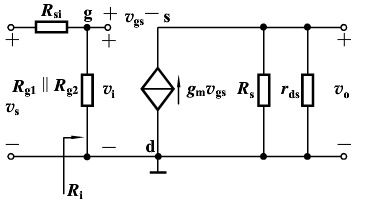
\includegraphics[width=0.5\linewidth]{figures/MOSFET-Common-Ds}
  \label{fig:}
\end{figure}

\begin{equation*}
  \begin{aligned}
    A_v = \dfrac{g_m \left( R_s \parallel r_{ds} \right)}{1 + g_m \left( R_s \parallel r_{ds} \right)} \approx 1
  \end{aligned}
\end{equation*}

\begin{equation*}
  \begin{aligned}
    R_i &= R_{g1} \parallel R_{g2} \\
    R_o &= R_s \parallel r_{ds} \parallel \dfrac{1}{g_m} 
  \end{aligned}
\end{equation*}


\subsection{Common Gate Amplifier Circuit}

\begin{figure}[H]
  \centering
  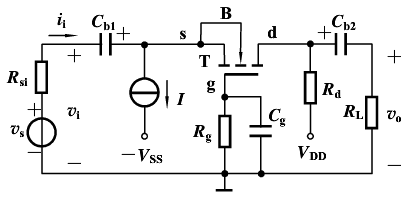
\includegraphics[width=0.5\linewidth]{figures/MOSFET-Common-G}
  \label{fig:}
\end{figure}

\begin{equation*}
  \left\{
  \begin{aligned}
    I_{DQ} &= K_n \left( V_{GSQ} - V_{TN} \right)^2 = I\\
    V_{DSQ} &= V_{DD} - I_{DQ} R_d + V_{GSQ}
  \end{aligned}
  \right.
\end{equation*}

\begin{equation*}
  \begin{aligned}
    g_m = 2 K_n \left( V_{GSQ} - V_{TN} \right)
  \end{aligned}
\end{equation*}

\begin{figure}[H]
  \centering
  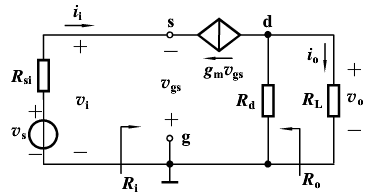
\includegraphics[width=0.5\linewidth]{figures/MOSFET-Common-Gs}
  \label{fig:}
\end{figure}

\begin{equation*}
  \begin{aligned}
    A_v = g_m \left( R_d \parallel R_L \right)
  \end{aligned}
\end{equation*}
\begin{equation*}
  \begin{aligned}
    R_i &\approx \dfrac{1}{g_m} \\
    R_o &\approx R_d
  \end{aligned}
\end{equation*}




%%% Local Variables:
%%% mode: latex
%%% TeX-master: "main"
%%% End:
